\documentclass{amsart}
\input{decls}
\title{Graphs}
\author{Frank Tsai}
\date{\today}
%\thanks{}
\begin{document}
\maketitle
\tableofcontents

\section{Graphs}
\label{sec:graphs}

\begin{defn}
  \label{defn:graphs}
  A (directed) \emph{graph} $G$ consists of the following data:
  \begin{enumerate}
  \item A set $V$ of \emph{vertices}.
  \item A set $E \subseteq V \times V$ of \emph{edges}.
  \end{enumerate}
\end{defn}

\begin{rmk}
  \label{rmk:edges-are-binary-relations}
  Recall that a binary relation on a set $V$ can be encoded as any subset of $V \times V$.
  Thus, a graph is a set $V$ equipped with a binary relation $E$.
\end{rmk}

\begin{eg}
  \label{eg:graphs-example1}
  Let $V = \{A, B, C\}$ and $E = \{(A,B),(B,A),(B,C),(C,A)\}$.
  \begin{center}
    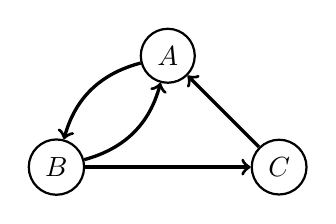
\begin{tikzpicture}[node distance= 2cm]
      \begin{scope}[every node/.style={circle,thick,draw}]
        \node (A) {$A$};
        \node (B) [below left of= A] {$B$};
        \node (C) [below right of=A] {$C$};
      \end{scope}
      \begin{scope}[every edge/.style={draw= black, very thick}]
        \path[->] (A) edge[bend right= 30] (B);
        \path[->] (B) edge[bend right= 30] (A);
        \path[->] (B) edge (C);
        \path[->] (C) edge (A);
      \end{scope}
    \end{tikzpicture}
  \end{center}
\end{eg}

\begin{defn}
  \label{defn:graphs-undirected}
  A graph $(V,E)$ is \emph{undirected} if the binary relation $E$ is symmetric.
\end{defn}

\begin{rmk}
  \label{rmk:example1-not-undirected}
  \cref{eg:graphs-example1} is not an undirected graph since $(B,C) \in E$, but $(C,B) \notin E$.
  Similarly, $(C,A) \in E$, but $(A,C) \notin E$.
\end{rmk}

\begin{rmk}
  \label{rmk:drop-arrows-in-undirected-graphs}
  In an undirected graph, we drop the arrow tips as they convey no additional information.
\end{rmk}

\begin{eg}
  \label{eg:graphs-example2}
  Let $V = \{A, B, C\}$ and $E = V \times V$.
  Note that $E$ is symmetric.
  \begin{center}
    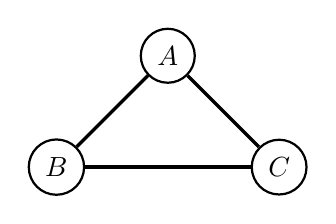
\begin{tikzpicture}[node distance= 2cm]
      \begin{scope}[every node/.style={circle,thick,draw}]
        \node (A) {$A$};
        \node (B) [below left of= A] {$B$};
        \node (C) [below right of=A] {$C$};
      \end{scope}
      \begin{scope}[every edge/.style={draw= black, very thick}]
        \path (A) edge (B);
        \path (A) edge (C);
        \path (B) edge (C);
      \end{scope}
    \end{tikzpicture}
  \end{center}
\end{eg}

\begin{defn}
  Let $G$ be a graph.
  A \emph{walk} is a sequence of vertices and edges defined inductively as follows:
  \begin{enumerate}
  \item If $(v_{1},v_{2}) \in E$ then the sequence $v_{1},(v_{1},v_{2}),v_{2}$ is a walk.
  \item If $(v_{n}, v_{m}) \in E$ and $v_{1},(v_{1},v_{2}),v_{2},\ldots,v_{n}$ is a walk then $v_{1},(v_{1},v_{2}),v_{2},\ldots,v_{n},(v_{n},v_{m}),v_{m}$ is a walk.
  \end{enumerate}
\end{defn}

\begin{eg}
  \label{eg:walk-example1}
  Let $G$ be the graph defined in \cref{eg:graphs-example2}.
  The sequence
  \[
    A,(A,B),B,(B,C),C,(C,A),A,(A,B),B
  \]
  is a walk.
  \begin{center}
    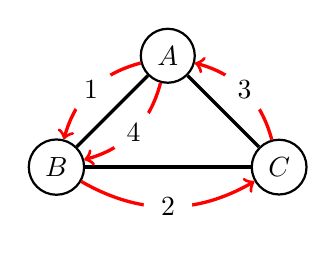
\begin{tikzpicture}[node distance= 2cm]
      \begin{scope}[every node/.style={circle,thick,draw}]
        \node (A) {$A$};
        \node (B) [below left of= A] {$B$};
        \node (C) [below right of=A] {$C$};
      \end{scope}
      \begin{scope}
        [every edge/.style={draw= black, very thick},
        every node/.style={fill=white,circle}]
        \path (A) edge (B);
        \path (A) edge (C);
        \path (B) edge (C);
        \path[->] (A) edge[draw= red, bend right= 30] node {$1$} (B);
        \path[->] (B) edge[draw= red, bend right= 30] node {$2$} (C);
        \path[->] (C) edge[draw= red, bend right= 30] node {$3$} (A);
        \path[->] (A) edge[draw= red, bend left= 30] node {$4$} (B);
      \end{scope}
    \end{tikzpicture}
  \end{center}
  Each red arrow represents a step of the walk.
\end{eg}

\section{BFS}
\label{sec:bfs}

\section{DFS}
\label{sec:dfs}



\end{document}
